\documentclass[12pt]{article}
\usepackage{graphicx}
\usepackage{hyperref}
\usepackage{amsmath}
\usepackage{titlesec}
\usepackage{caption} 
\usepackage{float}
\usepackage{fancyhdr}
\usepackage{algorithm}
\usepackage{algpseudocode}
\usepackage{subcaption}
\pagestyle{fancy}
\titleformat{\section}{\normalfont\Large\bfseries}{}{0em}{}
\titleformat{\subsection}{\normalfont\large\bfseries}{}{0em}{}

\usepackage{fancyhdr}
\pagestyle{fancy}
\fancyhf{}
\rhead{Query Processing and Optimization in SQL}
\lhead{Team PRQL}
\rfoot{\thepage}

\usepackage[top=1in, bottom=0.8in, left=0.6in, right=0.6in]{geometry}
\setlength{\headwidth}{\paperwidth}
\addtolength{\headwidth}{-1.2in}

\title{\bfseries Query Processing and Optimization in SQL}

\author{
  \begin{tabular}{ccccc}
    Rishit Garg & Nived Shah & Harshit Jain & Sachish Singla & Parth Patil \\
    {\small 22CS30045} & {\small 22CS10049} & {\small 22CS10030} & {\small 22CS30046} & {\small 22CS30041} \\
  \end{tabular}
  \\\\[1em]
  \textbf{Team PRQL}
}


\date{}


\date{}

\begin{document}

\maketitle

\begin{abstract}

As the scale of data in modern applications continues to grow, inefficient SQL queries can become significant bottlenecks in database performance. This project aims to implement a custom SQL query optimization system that enhances query execution by integrating parsing, relational algebra transformations, and cost-based optimization strategies. The system is designed to demonstrate practical applications of classical database optimization techniques.
\end{abstract}

\begin{figure}[h]
  \centering
  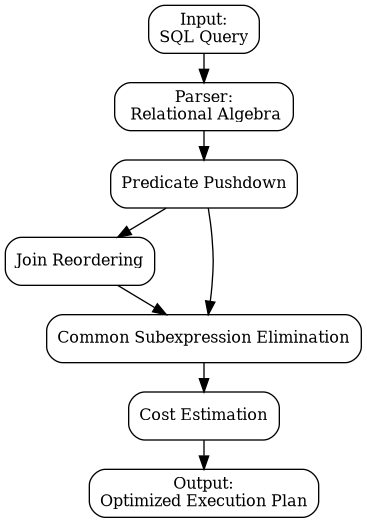
\includegraphics[width=0.4\textwidth]{images/sql_optimizer_flow.png}
  \caption{Query Optimization Pipeline}\label{fig:pipeline}
  \label{fig:flow}
\end{figure}


\section*{Methodology}

This system was architected with a modular, layered approach to enable effective, step-wise SQL query optimization. Each component focuses on a distinct optimization technique, working together to transform raw SQL input into an optimized relational algebra plan. \textbf{PostgreSQL} plays a central role in this pipeline as a source of crucial statistical metadata used in \textbf{cost-based decisions}.
The end-to-end pipeline begins with SQL parsing and proceeds through logical transformations such as predicate pushdown and common subexpression elimination, culminating in a cost-based join optimization step. At each stage, intermediate plans are visualized using a web interface. For an overview of the full pipeline, refer to Figure~\ref{fig:pipeline}.

\subsection*{1. SQL Parser}

The SQL parser is the first component of the query optimization pipeline. Its main function is to tokenize SQL queries and transform them into a machine-readable structure: a \textbf{relational algebra tree} represented in \textbf{JSON format}. This structured output forms the basis for all subsequent optimizations.

\subsubsection*{Tools Used:}

\begin{itemize}
    \item \textbf{Flex}: Tokenizes the raw SQL input by breaking it down into meaningful units such as keywords (\texttt{SELECT}, \texttt{FROM}, \texttt{WHERE}), identifiers (table/column names), operators, and literals.
    \item \textbf{Bison}: Uses a context-free grammar to recognize SQL syntax and build an abstract syntax tree (AST). The AST is then transformed into a relational algebra JSON.
\end{itemize}

\subsubsection*{Supported SQL Subset}

The parser currently supports a meaningful subset of SQL that includes:
\begin{itemize}
    \item Basic \texttt{SELECT-FROM-WHERE} queries
    \item Simple \texttt{JOIN}s (using \texttt{ON} operator)
    \item Nested subqueries
\end{itemize}


\captionsetup{type=table}
\noindent\textbf{Example SQL Query Input and Output}
\begin{verbatim}
SELECT L.L_ORDERKEY, L.L_PARTKEY
FROM LINEITEM L
WHERE L.L_SHIPDATE >= '1994-01-01'
\end{verbatim}

% JSON Output Block
\begin{table}[H]
\captionsetup{type=table}
\begin{verbatim}
{
  "condition": {
    "left": {
      "attr": "L_SHIPDATE",
      "table": "L"
    },
    "right": {
      "type": "string",
      "value": "1994-01-01"
    },
    "type": "GE"
  },
  "input": {
    "columns": [
      {
        "attr": "L_ORDERKEY",
        "table": "L"
      },
      {
        "attr": "L_PARTKEY",
        "table": "L"
      }
    ],
    "input": {
      "tables": [
        {
          "alias": "L",
          "name": "LINEITEM"
        }
      ],
      "type": "table_scan"
    },
    "type": "project"
  },
  "type": "select"
}
\end{verbatim}
\end{table}

\subsection*{2. Predicate Pushdown}

The second phase of the query optimization pipeline focuses on a classical and highly effective transformation in relational algebra: \textbf{Predicate Pushdown}. 
This optimization rule aims to minimize the size of the data retrieved from the storage system. The rule reduces the size of data that are fetched by applying the filter (predicate) as near as possible to table scanning. This additionally reduces the size of intermediate results that optimize other operations such as JOIN.

\subsubsection*{Motivation}

In the original un-optimized query tree generated by the SQL parser, \texttt{Select} operations may appear higher up in the tree, often after expensive operations such as joins. Today, there is an increasing use of cloud-based and remote database systems, which calls for a method to reduce \textbf{network transfer latency} and data retrieval process (to provide a \textbf{higher degree of concurrency}). This is why Predicate Pushdown is an effective approach since it reduces the amount of data is fetched and transferred across the network from the remote host to the client. By moving down the selection condition closer to the relevant base tables so, the system:
\begin{itemize}
    \item Filters irrelevant rows early
    \item Shrinks the size of data being passed through joins or projections
    \item Reduces memory consumption and improves processing speed
\end{itemize}

\begin{algorithm}[H]
\caption{Predicate Pushdown Optimization}
\begin{algorithmic}
  \State \textbf{Input:} Logical query plan tree $T$
  \State \textbf{Output:} Optimized query plan with predicates pushed down

  \Function{Pushdown}{$T$}
    \If{$T$ is a leaf node (e.g., TableScan)}
      \State \Return $T$
    \EndIf

    \If{$T$ is a Select node with condition $C$ over subtree $S$}
      \State Decompose $C$ into conjunctive components $C_1 \land C_2 \land \dots \land C_n$
      \State $S \gets$ \Call{Pushdown}{$S$}
      \ForAll{$C_i$ in $\{C_1, C_2, \dots, C_n\}$}
        \State Identify the minimal subtree $S_i$ that contains all referenced attributes in $C_i$
        \State Push $C_i$ down to just above $S_i$
      \EndFor
      \State \Return Updated subtree with conditions pushed
    \Else
      \ForAll{child node $T_c$ of $T$}
        \State $T_c \gets$ \Call{Pushdown}{$T_c$}
      \EndFor
      \State \Return Updated node with pushed-down children
    \EndIf
  \EndFunction
\end{algorithmic}
\end{algorithm}


% \subsubsection*{Transformation Strategy}

% The optimizer walks through the tree recursively and identifies opportunities where the \texttt{Select} operator can be safely pushed down without changing the query’s semantics. This involves:
% \begin{itemize}
%     \item Analyzing selection conditions and determining which subtrees (tables) they refer to
%     \item Moving conditions closer to their respective \texttt{TableScan} nodes
%     \item Splitting compound conditions (e.g., conjunctive predicates with \texttt{AND}) into individual pushable components
% \end{itemize}
\subsubsection*{Example Query:}

\begin{verbatim}
SELECT L.L_ORDERKEY, L.L_PARTKEY
FROM LINEITEM L
JOIN ORDERS O ON L.L_ORDERKEY = O.O_ORDERKEY
WHERE L.L_SHIPDATE >= '1994-01-01' AND O.O_ORDERSTATUS = 'F'
\end{verbatim}

\vspace{-0.02in}
\begin{table}[H]
  \centering
   \begin{minipage}[t]{0.48\textwidth}
    \centering
    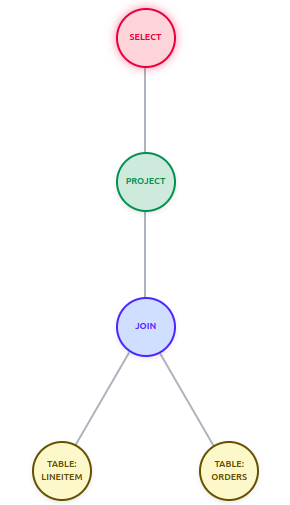
\includegraphics[width=0.6\textwidth]{images/pred_before.png}
    \captionof{figure}{Original Query Plan}
  \end{minipage}
  \hfill
  \begin{minipage}[t]{0.48\textwidth}
    \centering
    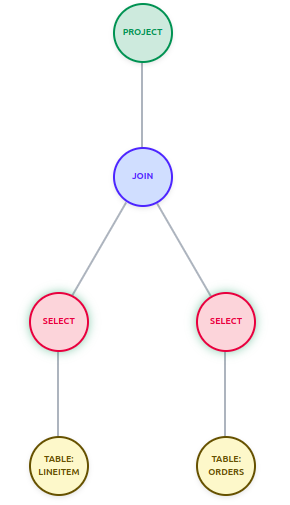
\includegraphics[width=0.6\textwidth]{images/pred_after.png}
    \captionof{figure}{After Predicate Pushdown}
  \end{minipage}
\end{table}

For a detailed explanation of the original and optimized query plans, refer to the appendix.

\subsection*{3. Join Optimizer}

The join optimizer is the most computation-intensive phase in the query optimization pipeline. It takes as input the optimized relational algebra tree (post predicate pushdown) in JSON format and outputs a reordered join plan that minimizes query execution cost using cost-based optimization.

\subsubsection*{Motivation}

Join operations are among the most expensive in SQL query processing. The order in which joins are executed can have a drastic impact on performance, especially for queries involving multiple tables. An inefficient join ordering may produce large intermediate results, whereas an optimal ordering can significantly reduce computation.

\subsubsection*{Join Predicate Graph Construction}

The optimizer first constructs a \textbf{join predicate graph}. This graph-based representation is crucial for understanding all relations involved and their predicate dependencies, including \textbf{implicit transitive joins} that might not be obvious from the original SQL.
To demonstrate, here is an example set of join predicates:
\begin{verbatim}
A JOIN B ON A.id = B.id2
B JOIN C ON B.id2 = C.id3
\end{verbatim}

\vspace{2em}
From the above, the optimizer infers that:
\begin{itemize}
    \item A joins with B (using \texttt{id2} of B)
    \item B joins with C (using \texttt{id2} of B)
    \item Therefore, A can indirectly join with C via B (transitive join)
\end{itemize}

This transitive inference allows the exploration of additional valid join paths (e.g., A-C) that may yield lower costs when reordered.

\begin{table}[h]
  \centering
   \begin{minipage}[t]{0.48\textwidth}
    \centering
    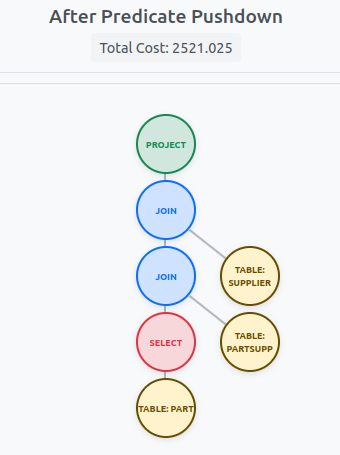
\includegraphics[width=\textwidth]{images/join_ex_before.png}
    \captionof{figure}{Original Query Plan}
  \end{minipage}
  \hfill
  \begin{minipage}[t]{0.48\textwidth}
    \centering
    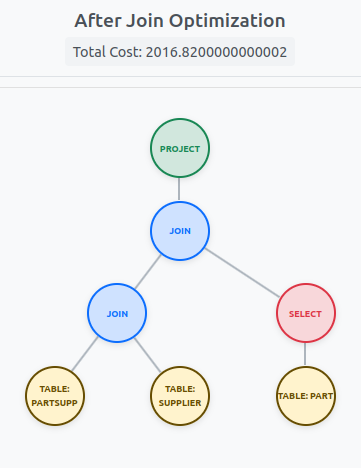
\includegraphics[width=\textwidth]{images/join_ex_after.png}
    \captionof{figure}{After Join Reordering}
  \end{minipage}
\end{table}

\subsubsection*{Join Order Enumeration and Strategy}

Once the join graph is built, the optimizer systematically explores all possible join orderings. For each valid order (based on tables permutations), it evaluates different join strategies and uses PostgreSQL’s statistics (from \texttt{`pg\_stat`}) to estimate cost.

\textbf{Steps:}
\begin{enumerate}
  \item \textbf{Cost Estimator Models:} Iterate through different models for cost estimation:
  \begin{itemize}
    \item \textbf{MCV (Most Common Value)} – focuses on skewed distributions
    \item \textbf{NDV (Number of Distinct Values)} – emphasizes cardinality spread
    \item \textbf{Fixed Estimates} – fallback with predefined selectivity assumptions
  \end{itemize}
  
  \item \textbf{Join Orderings:} Generate all valid permutations of table join sequences (e.g., ABC, ACB, BAC, etc.)
  
  \item \textbf{Join Tree Traversal:} For each order, simulate \textbf{left-deep join trees} using dynamic programming (Selinger-style):
  
  \begin{itemize}
    \item At each step, form a binary join node (R $\bowtie$ S)
    \item Use \textbf{PostgreSQL statistics} for R and S to calculate the node cost. 
  \end{itemize}
  
  \item \textbf{Join Strategies:} For each binary join:
  \begin{itemize}
    \item \textbf{Hash Join} – best when hashable keys exist
    \item \textbf{Nested Loop Join} – efficient for small tables
    \item \textbf{Block Nested Loop} – a middle ground strategy
  \end{itemize}

  \item \textbf{Cost Estimation:} Compute cost as a combination of:
  \begin{itemize}
    \item Estimated cardinality
    \item Disk I/O
    \item CPU usage
    \item Selectivity of predicates
  \end{itemize}

  \item \textbf{Dynamic Programming (Selinger's Algorithm):}
  \begin{itemize}
    \item Maintain a cost table mapping subplans to their best-known cost
    \item Reuse optimal subtrees to avoid recomputation
  \end{itemize}
\end{enumerate}

\begin{algorithm}[H]
\caption{Selinger-style Dynamic Programming Join Order Optimization}
\begin{algorithmic}
\State Initialize cost table $C$
\For{each single relation $R$}
    \State Set $C[\{R\}] = \text{cost}(R)$
\EndFor
\For{each join size $s = 2$ to $n$}
    \For{each subset $S$ of $s$ relations}
        \For{each partition of $S$ into $S_1$ and $S_2$}
            \State Compute cost of joining $C[S_1]$ and $C[S_2]$
            \State Update $C[S]$ if this plan is cheaper
        \EndFor
    \EndFor
\EndFor
\State Return optimal plan from $C[\text{all relations}]$
\end{algorithmic}
\end{algorithm}

\subsection*{4. Common Subexpression Elimination (CSE)}

In the context of relational algebra and SQL queries, common subexpressions typically arise when the same logical operations—such as selections, projections, or joins—are applied multiple times across different parts of a query.

\subsubsection*{Motivation}
Common Subexpression Elimination not only simplifies the logical representation of the query but also facilitates more efficient physical execution by allowing intermediate results to be computed once and reused.

\subsubsection*{Redundancy Detection}

The system traverses the relational algebra tree to identify structurally and semantically identical subtrees—i.e., common subexpressions. These subtrees are compared based on their operation types, inputs, and conditions, while trivial variations (e.g., different column names or aliases) are ignored. Only subtrees of sufficient depth and recurrence are considered meaningful for elimination. This process ensures that only computationally expensive or repeatedly occurring expressions are selected for optimization.

\subsubsection*{Replacement by References and DAG Construction}

Once redundancies are detected, each unique subexpression is abstracted and assigned a symbolic identifier. Every instance of the same expression in the tree is then replaced with a reference to this identifier. To support such reference-based reuse, the original tree structure is transformed into a Directed Acyclic Graph (DAG) following the steps below:

\begin{itemize} \item The tree is traversed in a bottom-up fashion. \item A structural hash is computed for each subtree to detect equivalence. \item When a match is found, the existing node is reused instead of duplicating it. \end{itemize}

This DAG representation allows the system to compute shared subexpressions only once, reducing redundancy, saving computation, and improving query execution efficiency without altering semantics.

\subsubsection*{Example Query:}

\begin{verbatim}
SELECT H.C_NAME, O.O_ORDERKEY, O.O_TOTALPRICE 
FROM (
  SELECT CUSTOMER.C_CUSTKEY, CUSTOMER.C_NAME, CUSTOMER.C_ACCTBAL 
  FROM CUSTOMER 
  WHERE CUSTOMER.C_ACCTBAL > 1000
) H
JOIN (
  SELECT CUSTOMER.C_CUSTKEY, CUSTOMER.C_NAME, CUSTOMER.C_ACCTBAL 
  FROM CUSTOMER 
  WHERE CUSTOMER.C_ACCTBAL > 1000
) I ON H.CUSTOMER.C_NATIONKEY = I.CUSTOMER.C_NATIONKEY
JOIN ORDERS O ON H.CUSTOMER.C_CUSTKEY = O.O_CUSTKEY 
WHERE O.O_TOTALPRICE > 50000 AND O.O_ORDERSTATUS = 'O' OR O.O_SHIPPRIORITY = 0
\end{verbatim}

\vspace{1em}

\begin{table}[H]
  \centering
   \begin{minipage}[t]{0.48\textwidth}
    \centering
    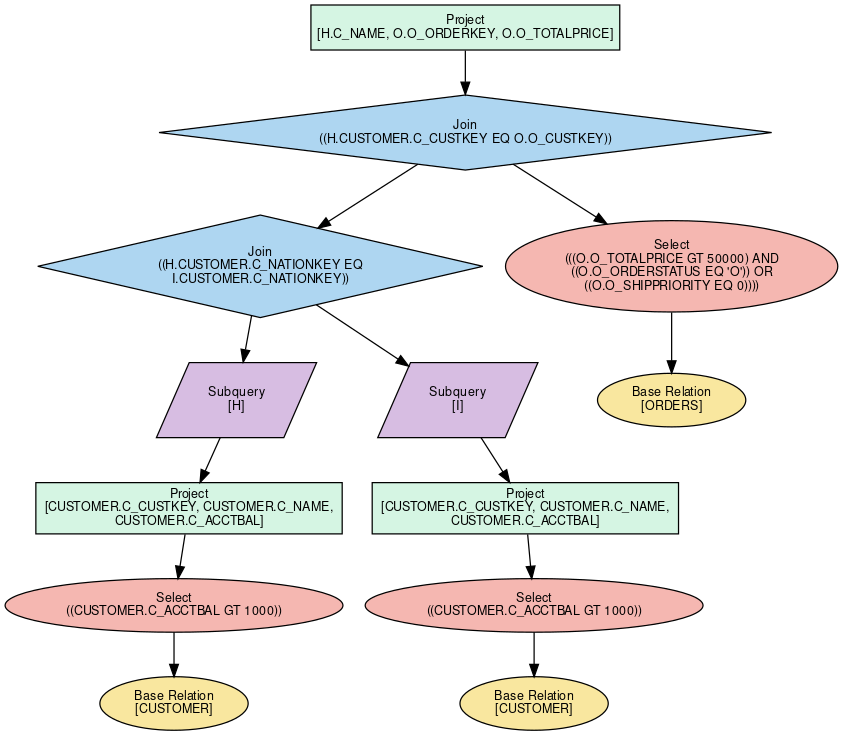
\includegraphics[width=0.8\textwidth]{images/cse_before.png}
    \captionof{figure}{After Predicate Pushdown}
  \end{minipage}
  \hfill
  \begin{minipage}[t]{0.48\textwidth}
    \centering
    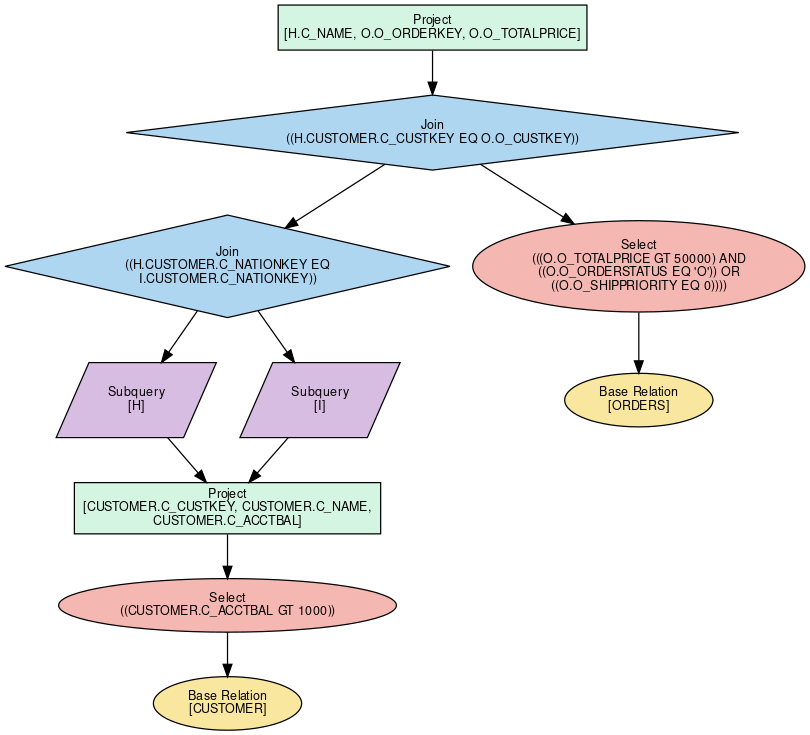
\includegraphics[width=0.8\textwidth]{images/cse_after.png}
    \captionof{figure}{After CSE}
  \end{minipage}
\end{table}


\subsection*{5. Web Interface for Visualization}

To facilitate user comprehension and interaction, an intuitive web interface was designed to visualize each stage of the SQL query optimization pipeline. This interface dynamically renders relational algebra trees corresponding to different phases: parsing, predicate pushdown, join reordering, and common subsequence elimination. Refer to the Appendix for screenshots of the User Interface.

\subsubsection*{Technologies Used}

\begin{itemize}
\item \textbf{Flask}: Serves as the backend framework, handling HTTP requests and responses, and orchestrating the flow between different optimization stages.
\item \textbf{Graphviz/JavaScript}: Generate visual representations of the relational algebra trees.
\item \textbf{HTML/CSS}: Construct the frontend, providing a responsive and interactive user interface.
\end{itemize}

\section*{Testing Methodology and Results}

To test the robustness and effectiveness of our Query Optimization system, we chose to use the schema provided in the \textbf{TPC-H Benchmark}. The schema has been provided in the appendix for reference. Since our system runs on a specific subset of queries, we chose to create our own set of 10 queries aimed at rigorously testing every aspect of the system. Overall, we acheived an average of \textbf{18\% reduction in cost}. 

\section*{Conclusion and Future Scope}

We have implemented a modular query optimization pipeline that processes SQL into relational algebra and applies classical and cost-based transformations. Each stage (parsing, pushdown, join ordering and common subexpression elimination) outputs JSON, facilitating debugging and extensibility. The system was tested on the TPC-H Benchmark for validation. The web interface built with Flask allows intuitive visualization of the entire optimization process.

\subsection*{Future Improvements:}
\begin{itemize}
  \item \textbf{Support for additional SQL constructs (e.g., GROUP BY, WITH)}: Such additional constructs give more variety of costing strategy that can be used to annotate the query plans.
  \item \textbf{Increasing query plan search space}: With the current approach, we find all possible Join Orders and evaluate the one with the least cost. However, cost-based optimization also includes generating all possible query plans considering other operators too, and finding the least cost plan amongst them.
  \item \textbf{Utilizing Machine Learning techniques for choosing cost parameters}: With knowledge of access history, the cost parameters such as predicate-selectivity can be predicted dynamically based on input query. This can be an interesting field to understand speed vs cost-prediction tradeoff since query fetching time must be fast, but including dynamicity for calculation may reduce speed. 
  \item \textbf{Understanding physical storage and Indexing support}: By default, Postgres can perform indexing based on primary-key. Identifying queries with use of primary-keys can enable use of Indexing to reduce cost. Additionally, strategies can be explored to create Indexes for high-volume data thus assisting clients to focus on abstract querying. This requires a thorough understanding of the physical storage used and data structures supported, and evaluating trade-offs between index creation cost and query processing cost dynamically.
\end{itemize}

\section*{References}

\begin{enumerate}
  \item Silberschatz, Korth, and Sudarshan. \textit{Database System Concepts}. 7th Edition.
  \item Jan Van den Bussche, Stijn Vansummeren. \textit{Translating SQL into the Relational Algebra}
  \item PostgreSQL Documentation: \url{https://www.postgresql.org/docs/}
  \item TPC-H Documentation: \url{https://www.tpc.org/tpch/default5.asp}
  \item tcph dbgen: \url{https://github.com/electrum/tpch-dbgen}
  \item Flask Documentation: \url{https://flask.palletsprojects.com/en/stable/}
  \item Graphviz Documentation: \url{https://graphviz.org/documentation/}
\end{enumerate}

\appendix

\section*{Appendix}

\subsection*{Screenshots of the User Interface}

\begin{figure}[H]
    \centering
    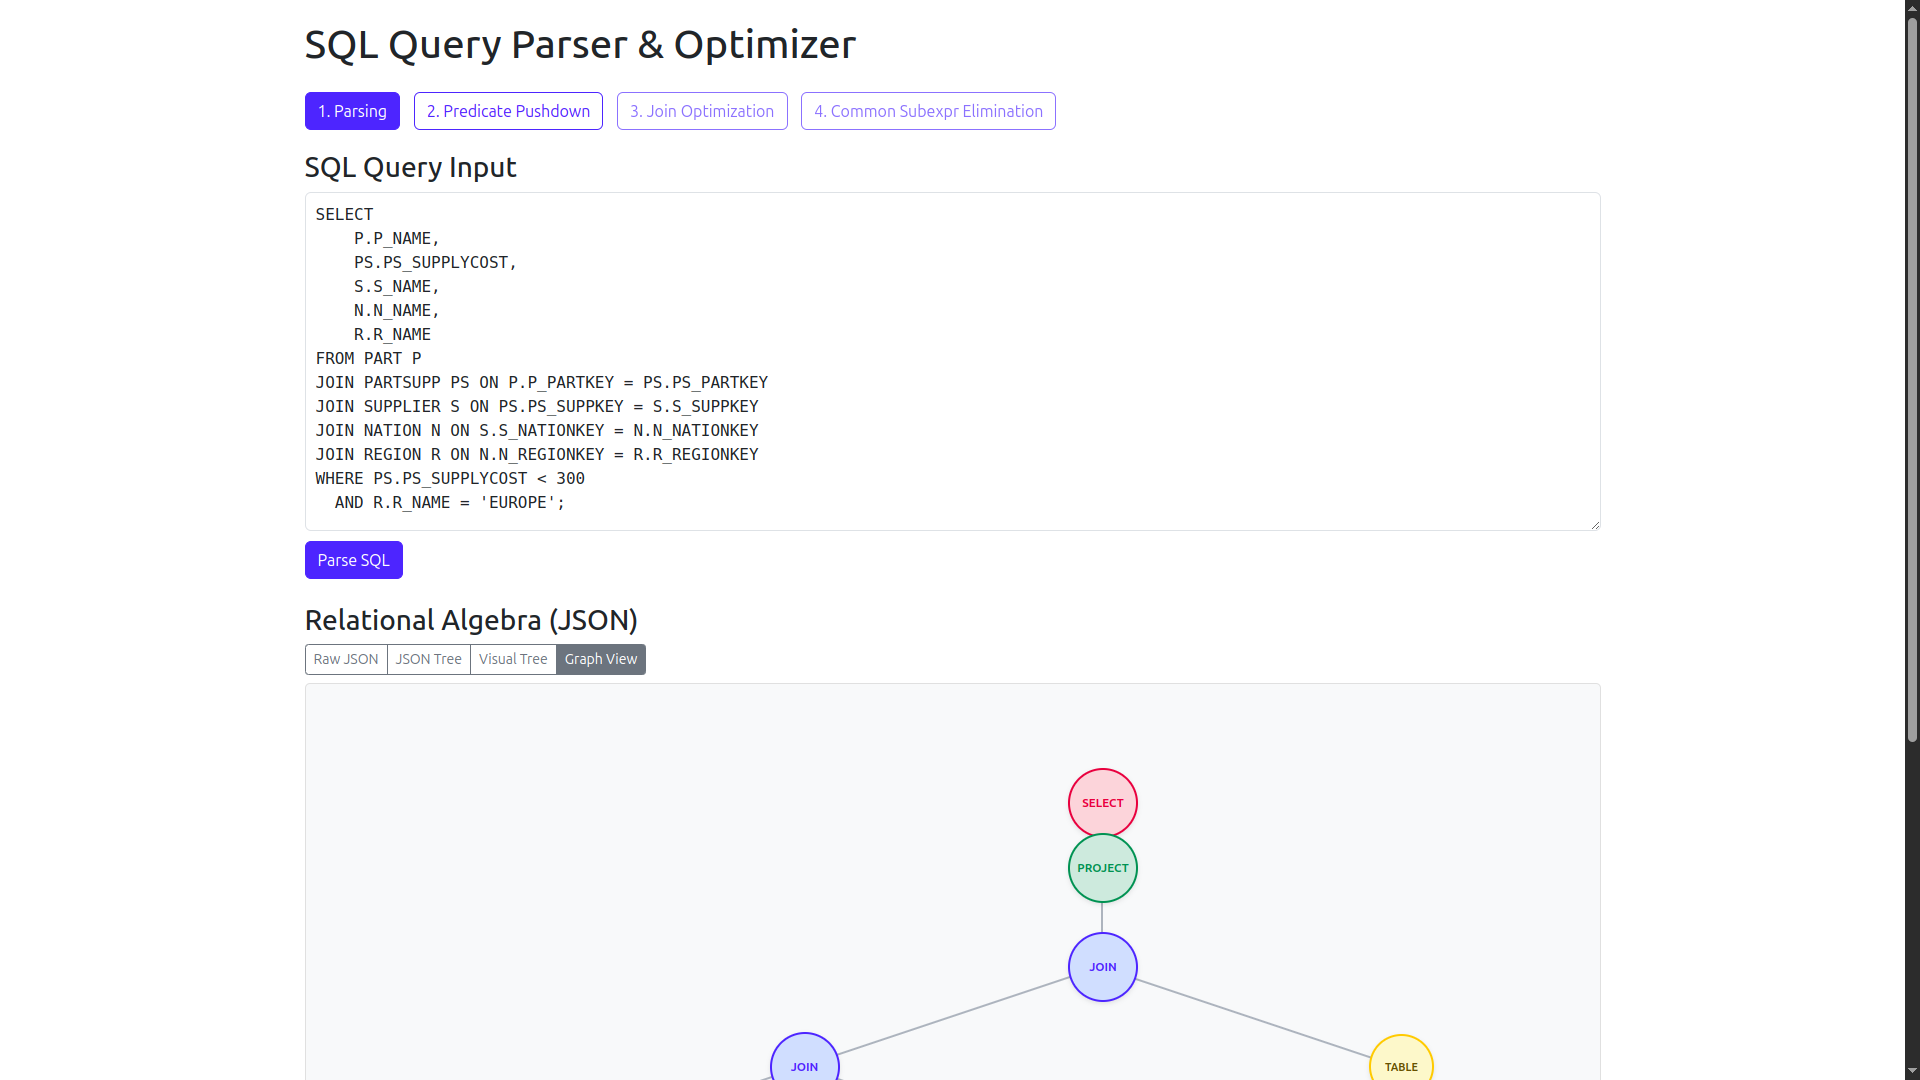
\includegraphics[width=0.85\textwidth]{images/ss1.png}
    \caption{Query Input}
\end{figure}

\begin{figure}[H]
    \centering
    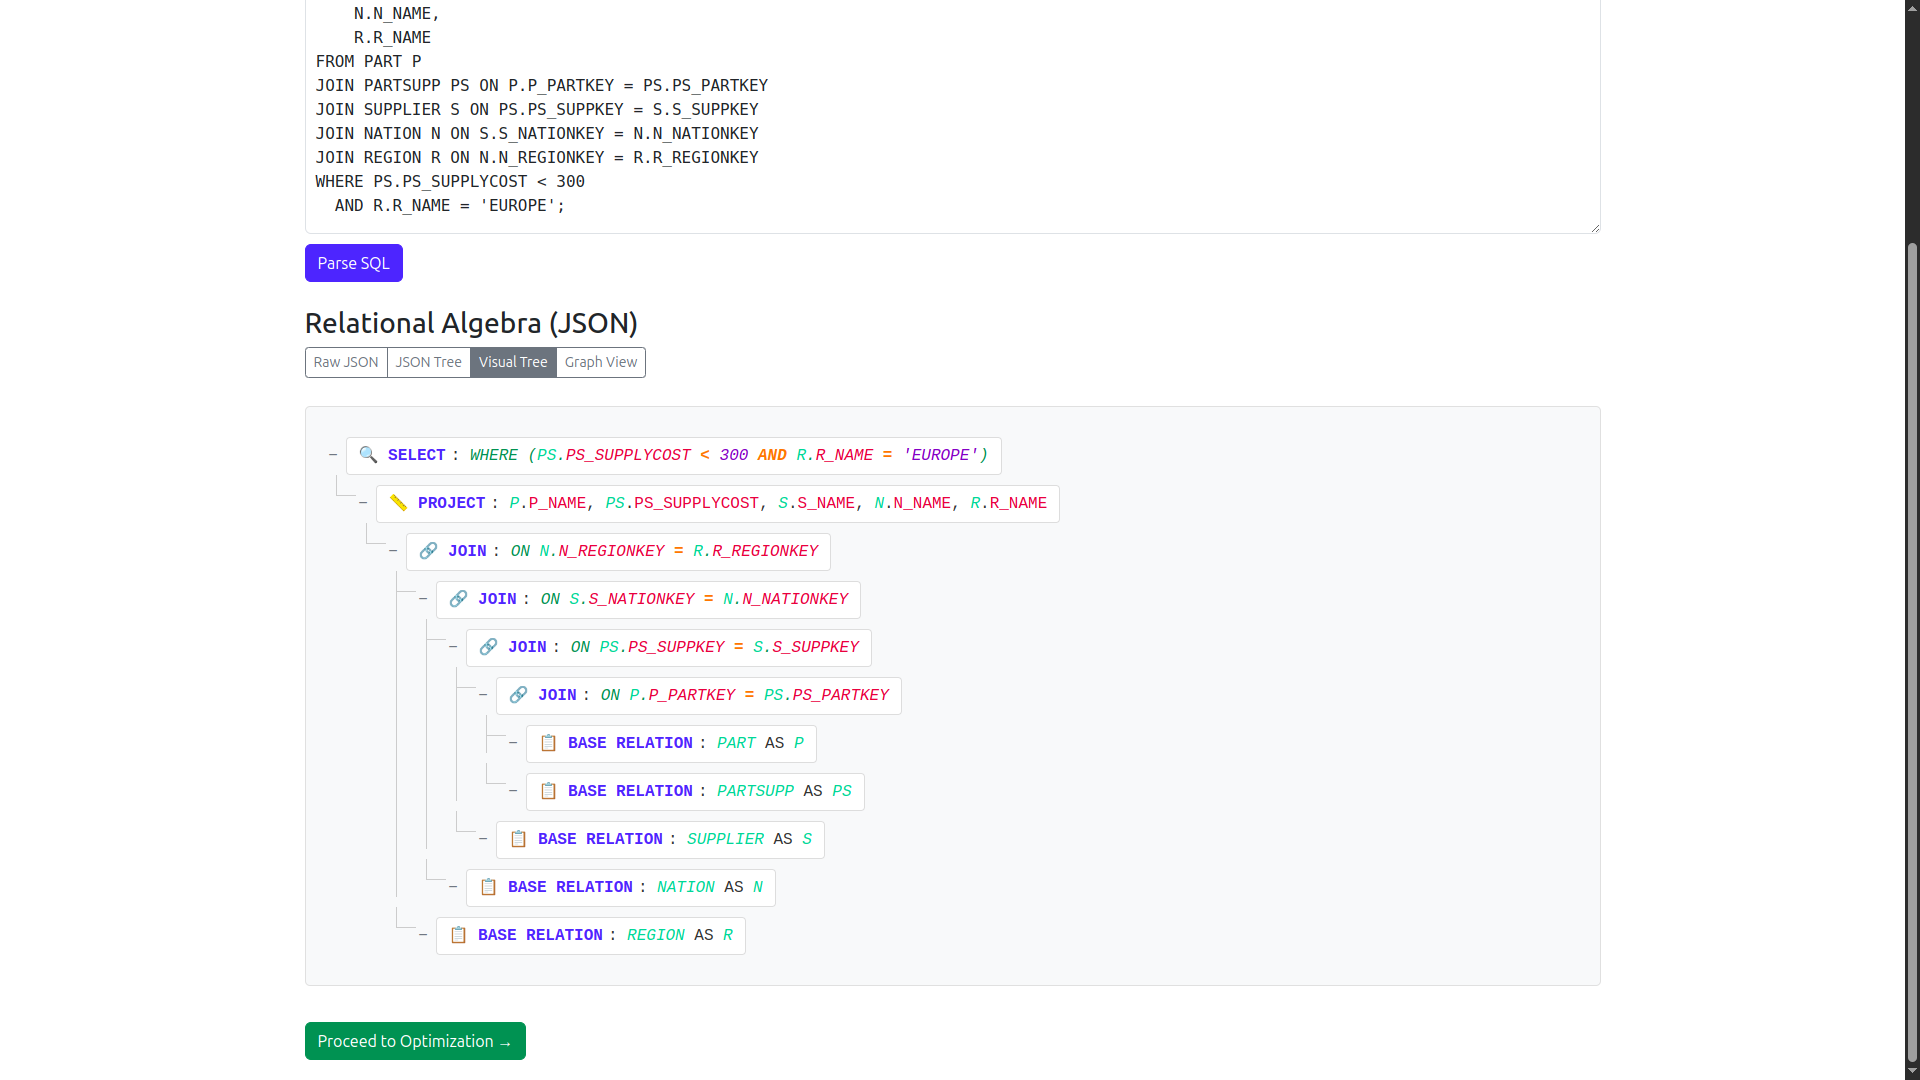
\includegraphics[width=0.85\textwidth]{images/ss2.png}
    \caption{Relational Algebra Output}
\end{figure}

\begin{figure}[H]
    \centering
    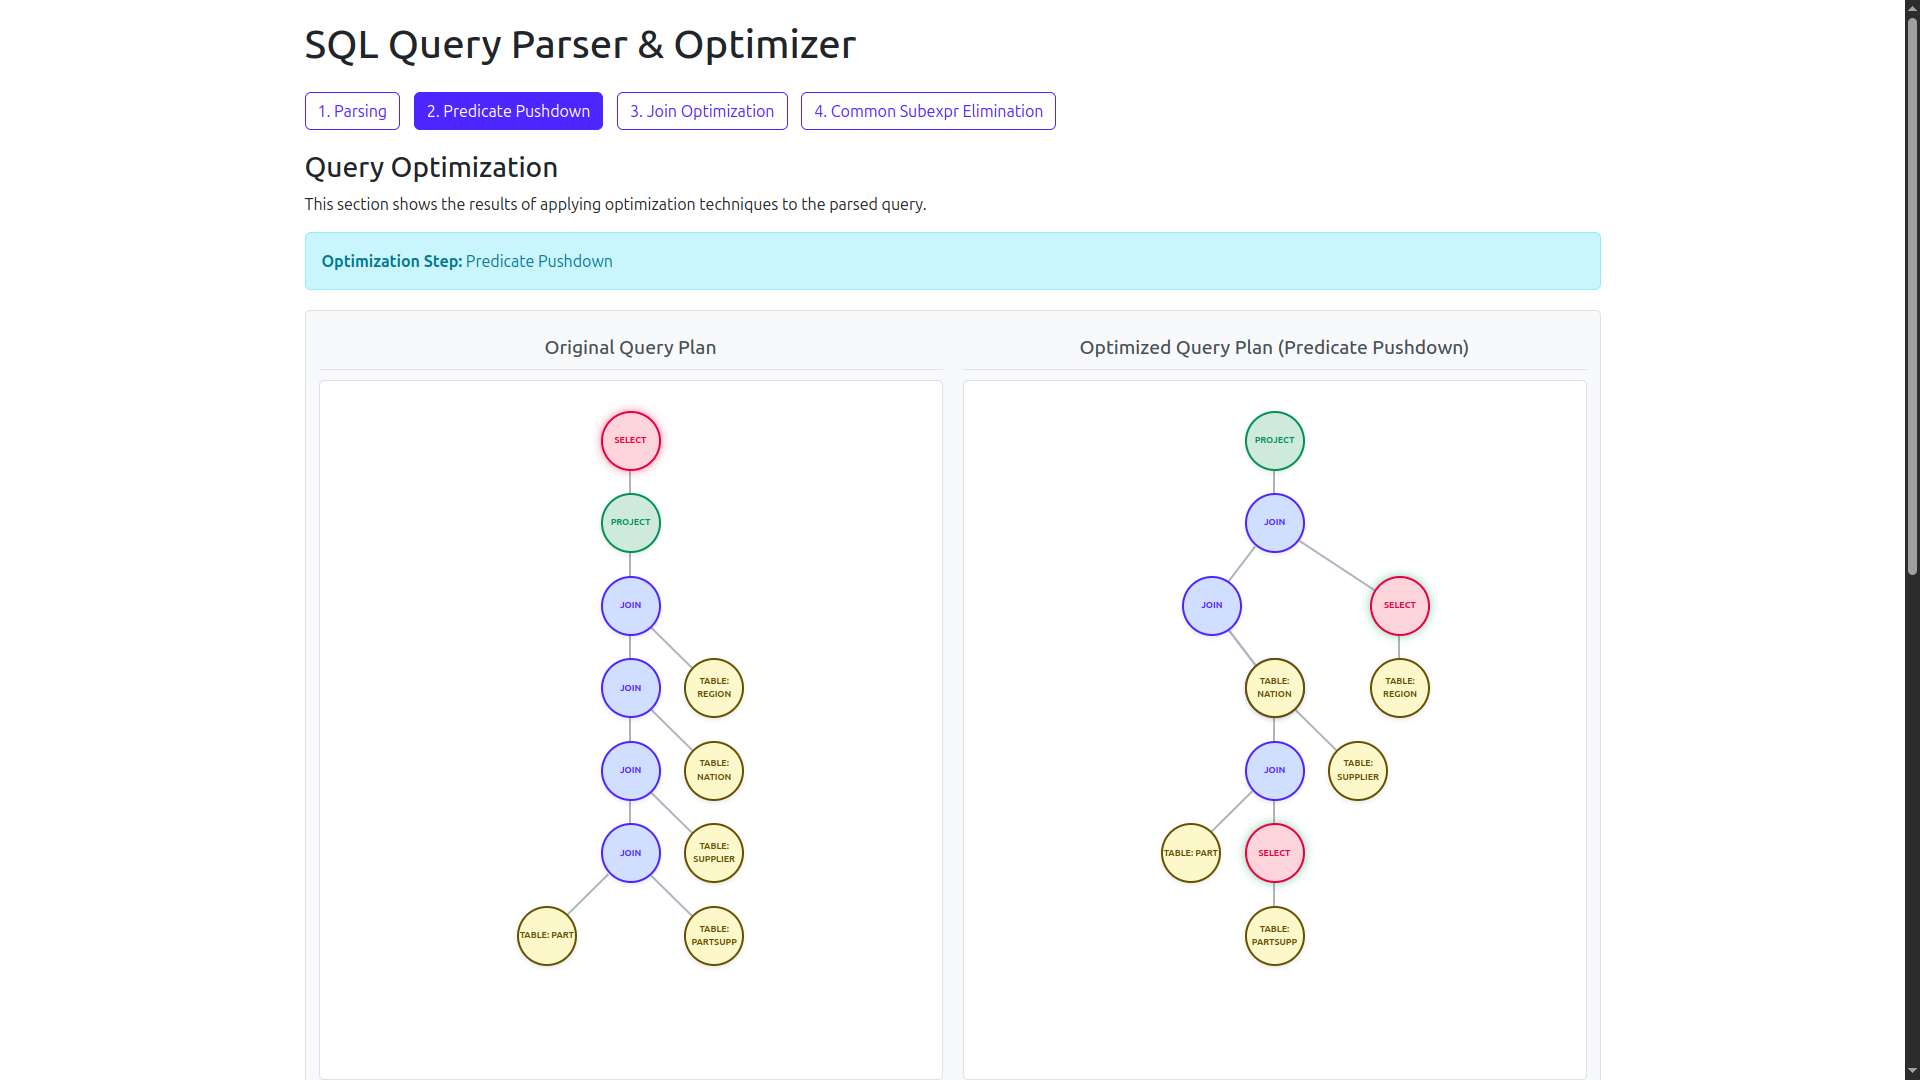
\includegraphics[width=0.85\textwidth]{images/ss3.png}
    \caption{Predicate Pushdown Trees}
\end{figure}

\begin{figure}[H]
    \centering
    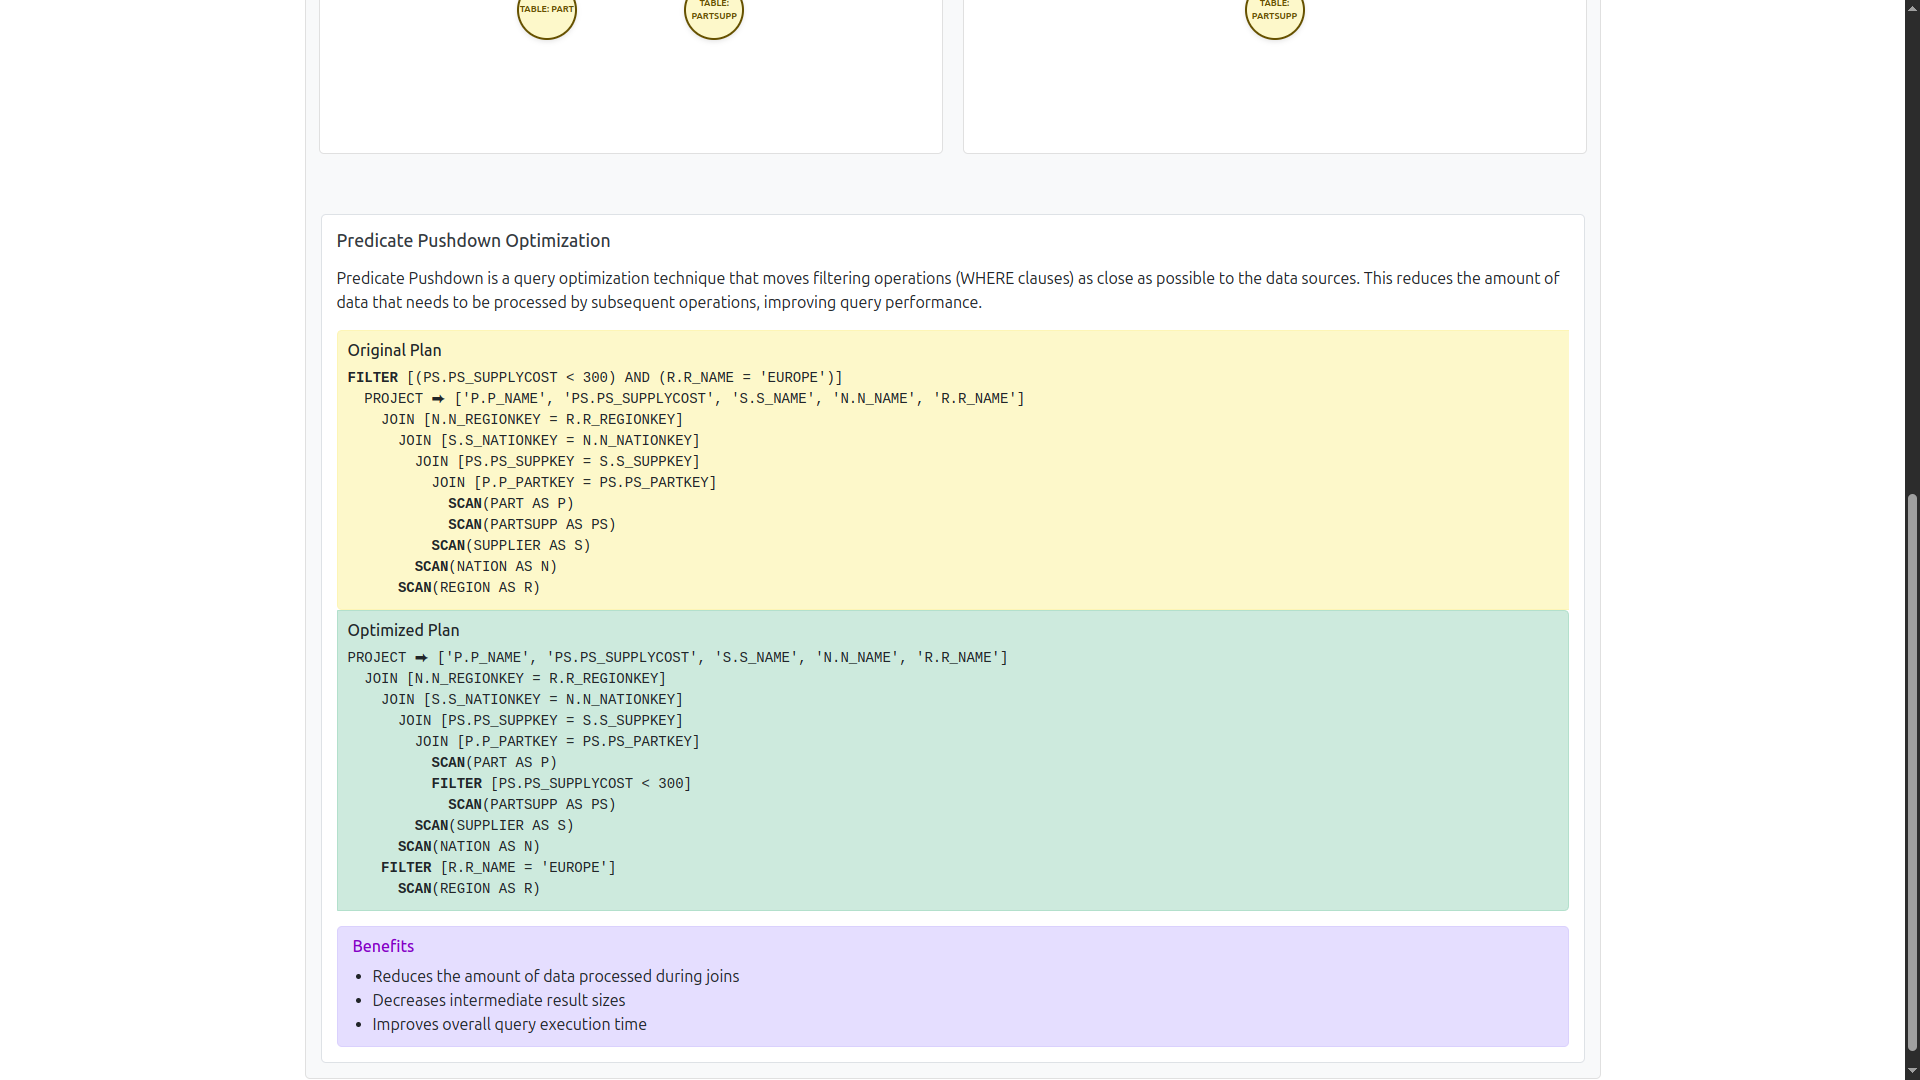
\includegraphics[width=0.85\textwidth]{images/ss4.png}
    \caption{Predicate Pushdown Description}
\end{figure}

\begin{figure}[H]
    \centering
    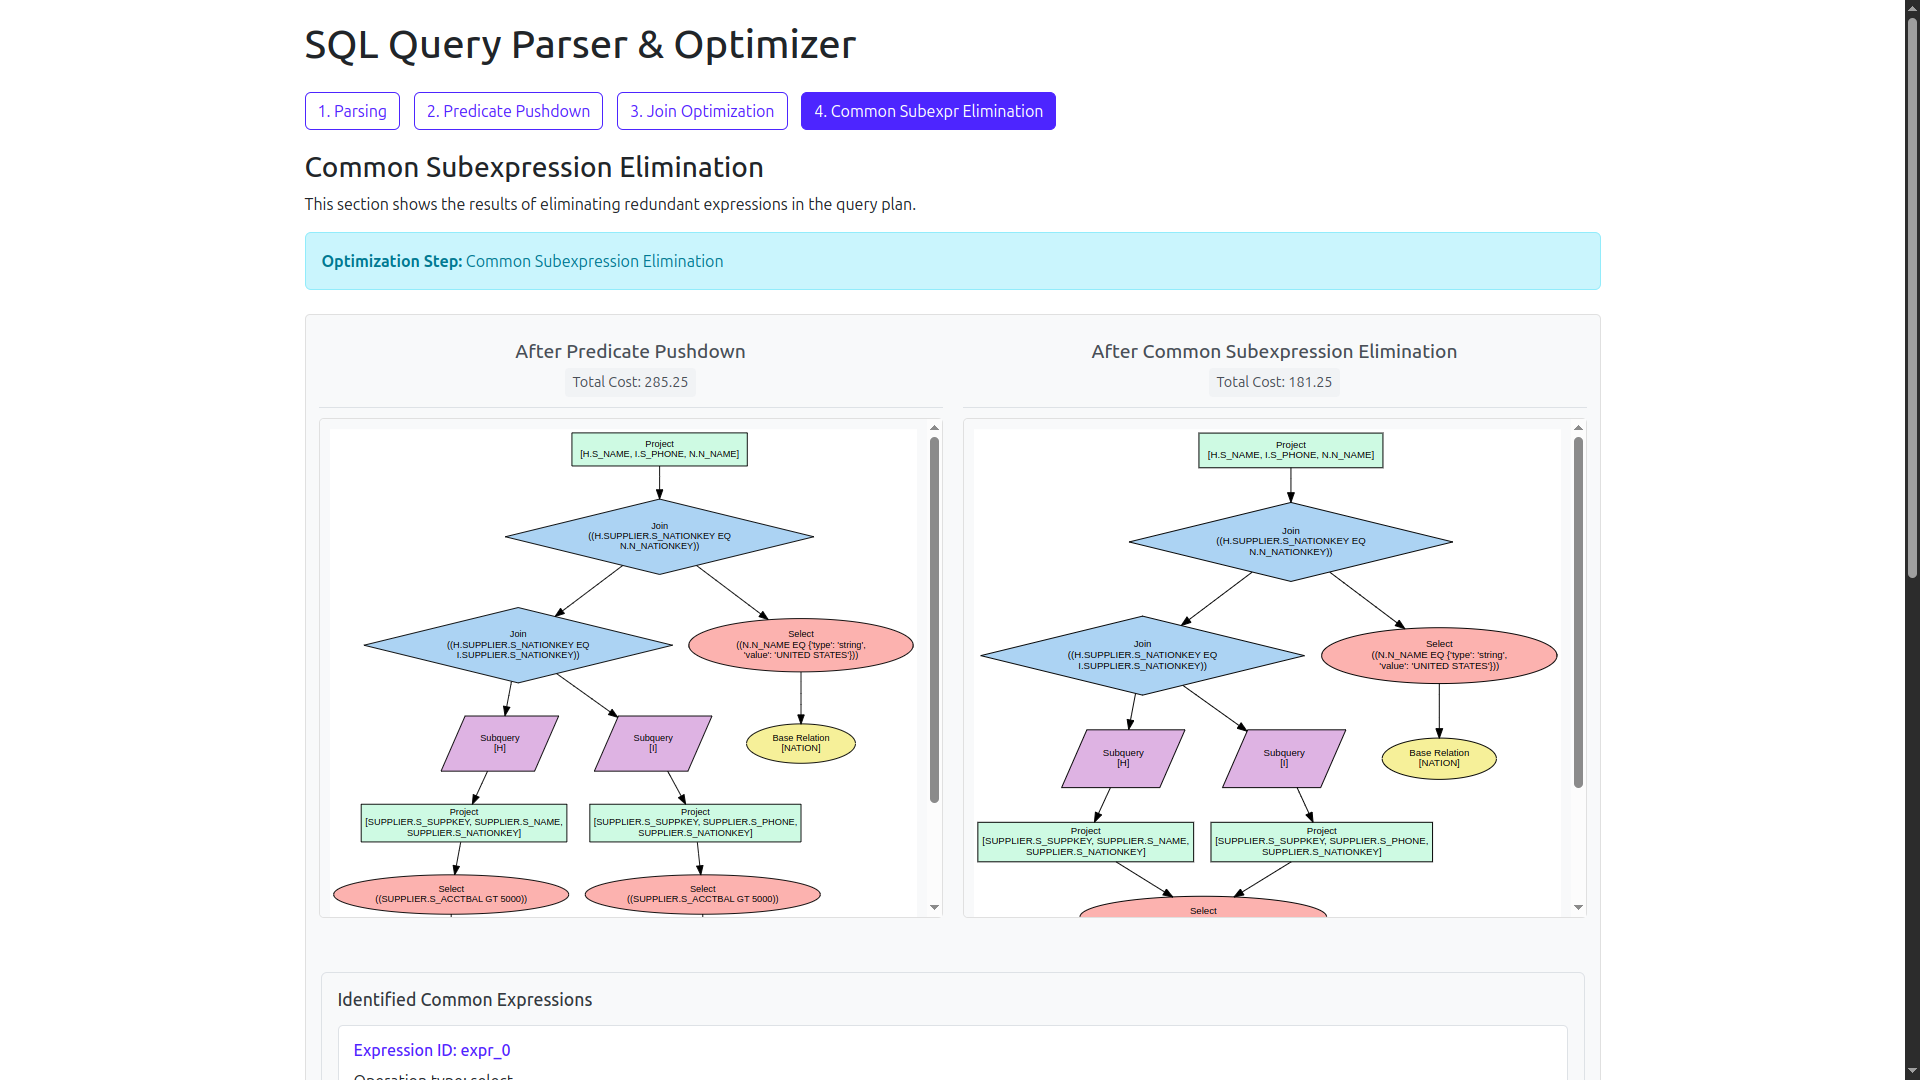
\includegraphics[width=0.85\textwidth]{images/ss5.png}
    \caption{Common Subexpression Elimination DAG}
\end{figure}

\begin{figure}[H]
    \centering
    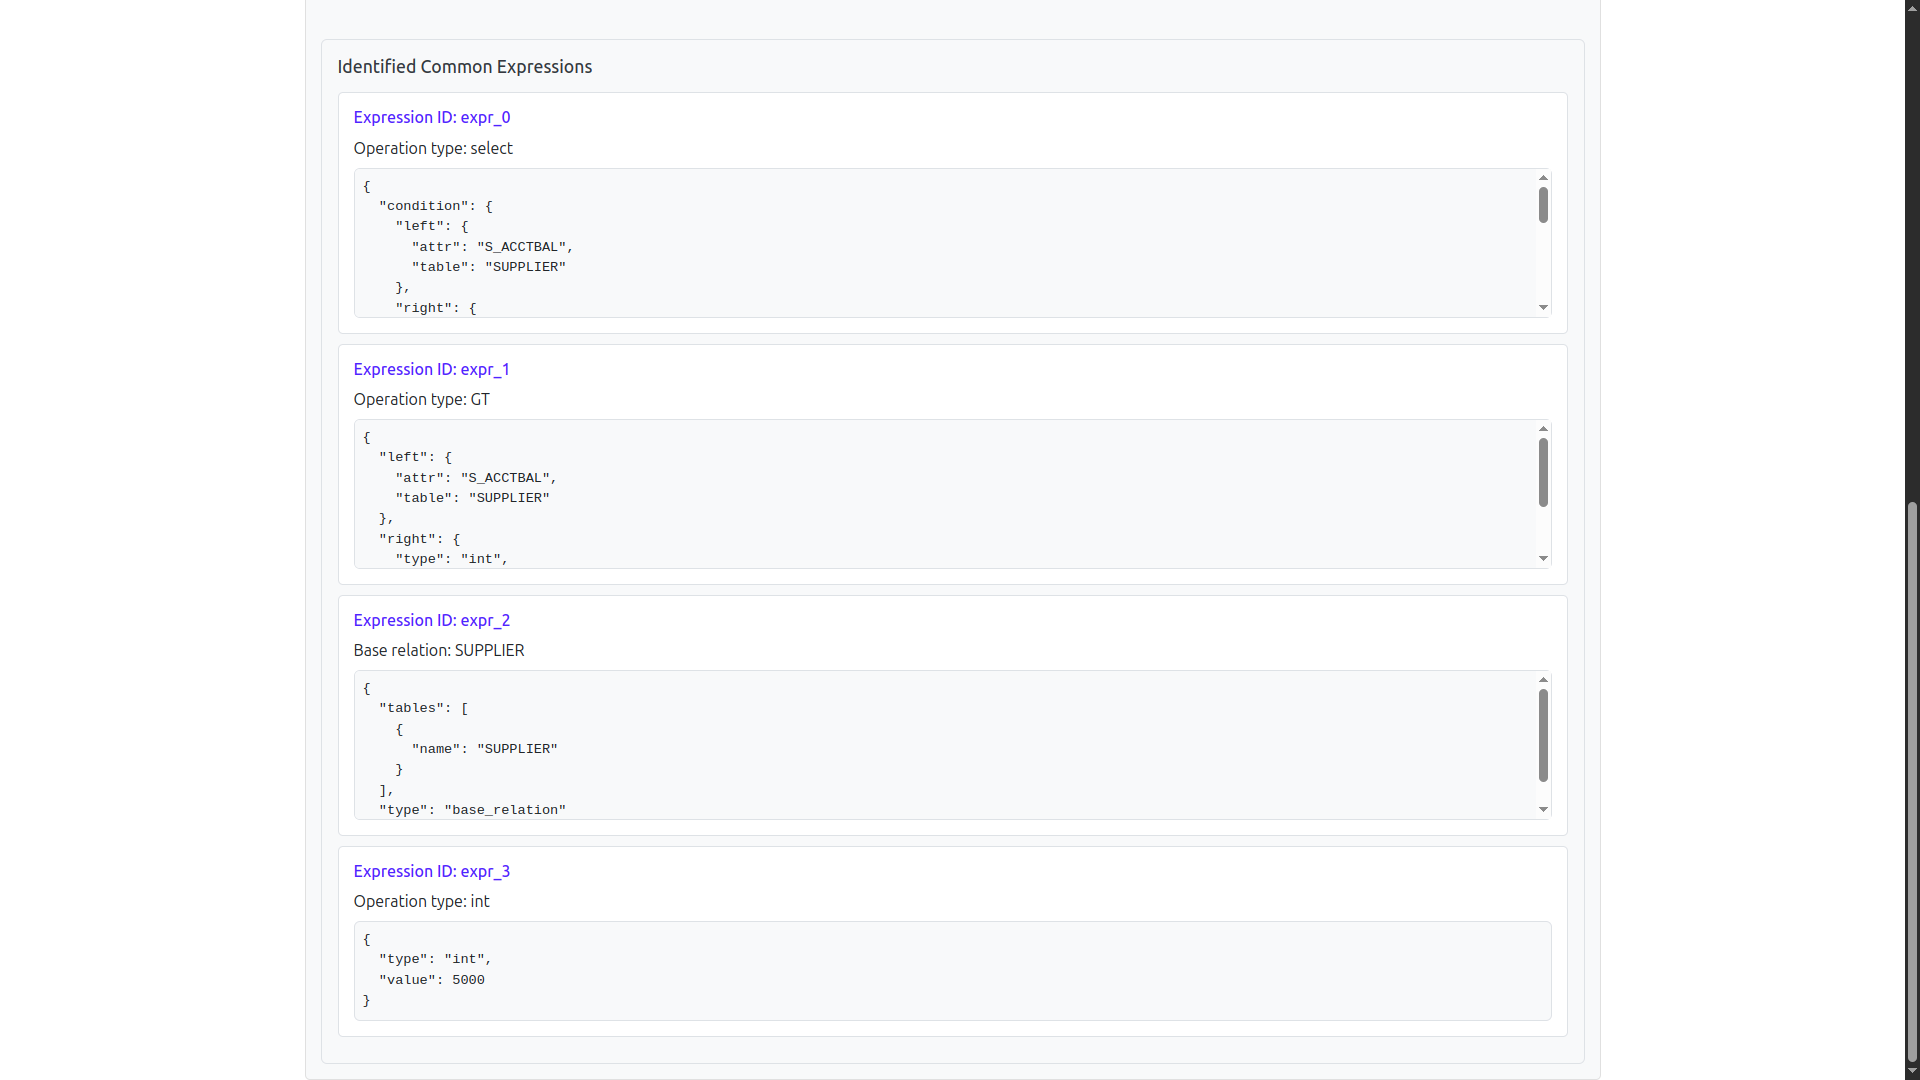
\includegraphics[width=0.85\textwidth]{images/ss6.png}
    \caption{Identified Common Subexpressions}
\end{figure}
\subsection*{Explanation of Predicate Pushdown Example}

Original Plan  
\begin{verbatim}
FILTER [(L.L_SHIPDATE >= '1994-01-01') AND (O.O_ORDERSTATUS = 'F')]
  PROJECT ['L.L_ORDERKEY', 'L.L_PARTKEY']
    JOIN [L.L_ORDERKEY = O.O_ORDERKEY]
      SCAN(LINEITEM AS L)
      SCAN(ORDERS AS O)
\end{verbatim}

Optimized Plan  
\begin{verbatim}
PROJECT ['L.L_ORDERKEY', 'L.L_PARTKEY']
  JOIN [L.L_ORDERKEY = O.O_ORDERKEY]
    FILTER [L.L_SHIPDATE >= '1994-01-01']
      SCAN(LINEITEM AS L)
    FILTER [O.O_ORDERSTATUS = 'F']
      SCAN(ORDERS AS O)
\end{verbatim}

\subsection*{TPC-H Schema}
\begin{verbatim}
CREATE TABLE NATION (
    N_NATIONKEY   INTEGER        NOT NULL,
    N_NAME        CHAR(25)       NOT NULL,
    N_REGIONKEY   INTEGER        NOT NULL,
    N_COMMENT     VARCHAR(152)
);
-----------------------------------------------------------------------------

CREATE TABLE REGION (
    R_REGIONKEY   INTEGER        NOT NULL,
    R_NAME        CHAR(25)       NOT NULL,
    R_COMMENT     VARCHAR(152)
);
-----------------------------------------------------------------------------

CREATE TABLE PART (
    P_PARTKEY     INTEGER        NOT NULL,
    P_NAME        VARCHAR(55)    NOT NULL,
    P_MFGR        CHAR(25)       NOT NULL,
    P_BRAND       CHAR(10)       NOT NULL,
    P_TYPE        VARCHAR(25)    NOT NULL,
    P_SIZE        INTEGER        NOT NULL,
    P_CONTAINER   CHAR(10)       NOT NULL,
    P_RETAILPRICE DECIMAL(15,2)  NOT NULL,
    P_COMMENT     VARCHAR(23)    NOT NULL
);
-----------------------------------------------------------------------------

CREATE TABLE SUPPLIER (
    S_SUPPKEY     INTEGER        NOT NULL,
    S_NAME        CHAR(25)       NOT NULL,
    S_ADDRESS     VARCHAR(40)    NOT NULL,
    S_NATIONKEY   INTEGER        NOT NULL,
    S_PHONE       CHAR(15)       NOT NULL,
    S_ACCTBAL     DECIMAL(15,2)  NOT NULL,
    S_COMMENT     VARCHAR(101)   NOT NULL
);
-----------------------------------------------------------------------------

CREATE TABLE PARTSUPP (
    PS_PARTKEY     INTEGER        NOT NULL,
    PS_SUPPKEY     INTEGER        NOT NULL,
    PS_AVAILQTY    INTEGER        NOT NULL,
    PS_SUPPLYCOST  DECIMAL(15,2)  NOT NULL,
    PS_COMMENT     VARCHAR(199)   NOT NULL
);
-----------------------------------------------------------------------------

CREATE TABLE CUSTOMER (
    C_CUSTKEY     INTEGER        NOT NULL,
    C_NAME        VARCHAR(25)    NOT NULL,
    C_ADDRESS     VARCHAR(40)    NOT NULL,
    C_NATIONKEY   INTEGER        NOT NULL,
    C_PHONE       CHAR(15)       NOT NULL,
    C_ACCTBAL     DECIMAL(15,2)  NOT NULL,
    C_MKTSEGMENT  CHAR(10)       NOT NULL,
    C_COMMENT     VARCHAR(117)   NOT NULL
);
-----------------------------------------------------------------------------

CREATE TABLE ORDERS (
    O_ORDERKEY       INTEGER        NOT NULL,
    O_CUSTKEY        INTEGER        NOT NULL,
    O_ORDERSTATUS    CHAR(1)        NOT NULL,
    O_TOTALPRICE     DECIMAL(15,2)  NOT NULL,
    O_ORDERDATE      DATE           NOT NULL,
    O_ORDERPRIORITY  CHAR(15)       NOT NULL,
    O_CLERK          CHAR(15)       NOT NULL,
    O_SHIPPRIORITY   INTEGER        NOT NULL,
    O_COMMENT        VARCHAR(79)    NOT NULL
);
-----------------------------------------------------------------------------

CREATE TABLE LINEITEM (
    L_ORDERKEY      INTEGER        NOT NULL,
    L_PARTKEY       INTEGER        NOT NULL,
    L_SUPPKEY       INTEGER        NOT NULL,
    L_LINENUMBER    INTEGER        NOT NULL,
    L_QUANTITY      DECIMAL(15,2)  NOT NULL,
    L_EXTENDEDPRICE DECIMAL(15,2)  NOT NULL,
    L_DISCOUNT      DECIMAL(15,2)  NOT NULL,
    L_TAX           DECIMAL(15,2)  NOT NULL,
    L_RETURNFLAG    CHAR(1)        NOT NULL,
    L_LINESTATUS    CHAR(1)        NOT NULL,
    L_SHIPDATE      DATE           NOT NULL,
    L_COMMITDATE    DATE           NOT NULL,
    L_RECEIPTDATE   DATE           NOT NULL,
    L_SHIPINSTRUCT  CHAR(25)       NOT NULL,
    L_SHIPMODE      CHAR(10)       NOT NULL,
    L_COMMENT       VARCHAR(44)    NOT NULL
);

\end{verbatim}

\subsection*{Benchmark Queries}

\begin{verbatim}
SELECT H.C_NAME, O.O_ORDERKEY, O.O_TOTALPRICE 
FROM (
  SELECT CUSTOMER.C_CUSTKEY, CUSTOMER.C_NAME, CUSTOMER.C_ACCTBAL 
  FROM CUSTOMER 
  WHERE CUSTOMER.C_ACCTBAL > 1000
) H
JOIN (
  SELECT CUSTOMER.C_CUSTKEY, CUSTOMER.C_NAME, CUSTOMER.C_ACCTBAL 
  FROM CUSTOMER 
  WHERE CUSTOMER.C_ACCTBAL > 1000
) I ON H.CUSTOMER.C_NATIONKEY = I.CUSTOMER.C_NATIONKEY
JOIN ORDERS O ON H.CUSTOMER.C_CUSTKEY = O.O_CUSTKEY 
WHERE O.O_TOTALPRICE > 50000 AND O.O_ORDERSTATUS = 'O' OR O.O_SHIPPRIORITY = 0;
-----------------------------------------------------------------------------

SELECT L.L_ORDERKEY, L.L_PARTKEY
FROM LINEITEM L
JOIN ORDERS O ON L.L_ORDERKEY = O.O_ORDERKEY
WHERE L.L_SHIPDATE >= '1994-01-01' AND O.O_ORDERSTATUS = 'F';
-----------------------------------------------------------------------------

SELECT P.P_NAME, P.P_BRAND
FROM PART P
JOIN PARTSUPP PS ON P.P_PARTKEY = PS.PS_PARTKEY
JOIN SUPPLIER S ON PS.PS_SUPPKEY = S.S_SUPPKEY
WHERE P.P_SIZE >= 25;
-----------------------------------------------------------------------------

SELECT S.S_NAME, N.N_NAME, L.L_EXTENDEDPRICE, O.O_ORDERDATE
FROM SUPPLIER S
JOIN NATION N ON S.S_NATIONKEY = N.N_NATIONKEY
JOIN LINEITEM L ON S.S_SUPPKEY = L.L_SUPPKEY
JOIN ORDERS O ON L.L_ORDERKEY = O.O_ORDERKEY
WHERE L.L_DISCOUNT > 0.05;
-----------------------------------------------------------------------------

SELECT 
    P.P_NAME,
    PS.PS_SUPPLYCOST,
    S.S_NAME,
    N.N_NAME,
    R.R_NAME
FROM PART P
JOIN PARTSUPP PS ON P.P_PARTKEY = PS.PS_PARTKEY
JOIN SUPPLIER S ON PS.PS_SUPPKEY = S.S_SUPPKEY
JOIN NATION N ON S.S_NATIONKEY = N.N_NATIONKEY
JOIN REGION R ON N.N_REGIONKEY = R.R_REGIONKEY
WHERE PS.PS_SUPPLYCOST < 300
  AND R.R_NAME = 'EUROPE';
-----------------------------------------------------------------------------

SELECT P.P_NAME, S.S_NAME, N.N_NAME, PS.PS_SUPPLYCOST
FROM PART P
JOIN PARTSUPP PS ON P.P_PARTKEY = PS.PS_PARTKEY
JOIN SUPPLIER S ON PS.PS_SUPPKEY = S.S_SUPPKEY
JOIN NATION N ON S.S_NATIONKEY = N.N_NATIONKEY
WHERE P.P_TYPE = 'COPPER'
  AND PS.PS_SUPPLYCOST < 500;
-----------------------------------------------------------------------------

SELECT H.S_NAME, I.S_PHONE, N.N_NAME
FROM (
  SELECT SUPPLIER.S_SUPPKEY, SUPPLIER.S_NAME, SUPPLIER.S_NATIONKEY
  FROM SUPPLIER
  WHERE SUPPLIER.S_ACCTBAL > 5000
) H
JOIN (
  SELECT SUPPLIER.S_SUPPKEY, SUPPLIER.S_PHONE, SUPPLIER.S_NATIONKEY
  FROM SUPPLIER
  WHERE SUPPLIER.S_ACCTBAL > 5000
) I ON H.SUPPLIER.S_NATIONKEY = I.SUPPLIER.S_NATIONKEY
JOIN NATION N ON H.SUPPLIER.S_NATIONKEY = N.N_NATIONKEY
WHERE N.N_NAME = 'UNITED STATES';
-----------------------------------------------------------------------------

SELECT O.ORDERKEY, L.QUANTITY, S.SUPPKEY, C.CUSTKEY
FROM ORDERS O 
JOIN CUSTOMER C ON O.CUSTKEY = C.CUSTKEY
JOIN LINEITEM L ON O.ORDERKEY = L.ORDERKEY
JOIN SUPPLIER S ON S.SUPPKEY = L.SUPPKEY
JOIN (SELECT N.NATIONKEY, N.NAME FROM NATION N) TMP1 ON TMP1.NATIONKEY = C.NATIONKEY
JOIN (SELECT N.NATIONKEY, N.NAME FROM NATION N) TMP2 ON TMP2.NATIONKEY = S.NATIONKEY;
-----------------------------------------------------------------------------

SELECT PS.PARTKEY, PS.SUPPLYKEY
FROM PARTSUPP PS 
JOIN SUPPLIER S ON PS.SUPPLYKEY = S.SUPPLYKEY
JOIN LINEITEM L ON PS.SUPPLYKEY = L.SUPPLYKEY
JOIN (SELECT P.NAME, P.BRAND FROM PART P) TMP1 ON TMP1.PARTKEY = PS.PARTKEY
JOIN (SELECT P.NAME, P.BRAND FROM PART P) TMP2 ON TMP2.PARTKEY = L.PARTKEY
WHERE PS.AVAILQTY > 10 AND S.ACCTBAL > 1000;
-----------------------------------------------------------------------------

SELECT P.PARTKEY, P.SUPPKEY
FROM PARTSUPP P
JOIN SUPPLIER S ON P.SUPPKEY = S.SUPPKEY
WHERE P.AVAILQTY > 10 OR P.SUPPLYCOST < 500 AND S.ACCTBAL > 1000;
-----------------------------------------------------------------------------
\end{verbatim}

\end{document}
